\subsection{核心协议的升级设计}

我们首先给出星云链中的区块结构,然后讨论如何在该区块结构上实现核心协议的升级问题。

\paragraph{区块结构}

星云链区块数据结构包含,但不限于以下信息:
\begin{itemize}
	\item Header:区块头
		\begin{itemize}
		\item Height:高度
		\item ParentHash:父区块哈希值
		\item Ts:时间戳
		\item Miner:记账人地址
		\item Dynasty:区块所处共识朝代
		\item Epoch:区块所处共识时代
		\item StateRoot:状态根哈希值
		\item TxsRoot:交易根哈希值
		\item ReceiptsRoot:交易收据根哈希值
		\item TransNum:交易数
		\end{itemize}
	\item Transactions:交易数据(包含多个交易)
		\begin{itemize}
		\item From:交易发起人地址
		\item To:交易接收人(普通用户或智能合约)地址,对于创建智能合约,值为0地址
		\item Value:转账金额
		\item Data:交易的payload。如果交易为创建智能合约,则为智能合约字节码;如果交易为智能合约调用,包含调用函数名称和入参值
		\item Signature:交易签名
		\item Gas:燃料上限
		\item GasPrice:燃料单价
		\item Nonce:标识交易唯一性
		\end{itemize}
	\item Votes:Prepare和Commit票数统计(包含多个),用在PoD(见\refsec{sec:pod})共识算法中
		\begin{itemize}
		\item From:投票人
		\item VoteHash:投票区块哈希
		\item Hv:投票区块所处高度
		\item Hvs:投票区块的某祖先高度
		\item VoteType:投票类型,Prepare或Commit
		\item Signature:投票签名
		\end{itemize}
	\item Protocol Code:核心协议代码(一个区块中只能有0或1个)
		\begin{itemize}
		\item Hash:哈希值
		\item Code:核心协议的字节码
		\item ValidStartBlock:协议生效起始区块号
		\item Signature:签名(校验是否来自开发者社区保留账号的签名)
		\item Version:标识核心协议版本号,每次升级都需要递增,防止恶意记账人回滚到老的Protocol Code
		\item Nonce:标识唯一性
		\end{itemize}
	\item Nebulas Rank:星云指数(计算周期为一周一次,大部分区块没有)
		\begin{itemize}
		\item RankVersion:NR版本
		\item RankRoot:NR排名哈希值
		\item RankRecords:NR排名记录
			\begin{itemize}
				\item Address:账号地址标记
				\item Score:NR值
			\end{itemize}
		\end{itemize}
\end{itemize}

\begin{figure}[h]
\centering
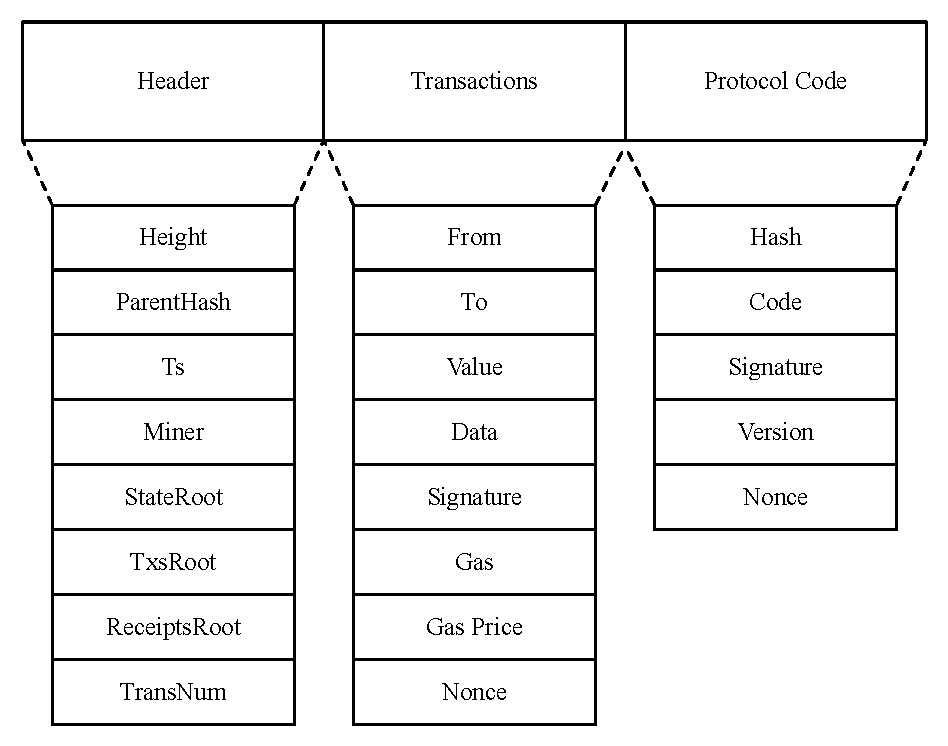
\includegraphics[width=13.8cm]{./figs/block}
\caption{区块结构}
\label{fig:block}
\end{figure}


类似于其他加密数字货币系统,用户和区块链上的互动都是通过特定的交易进行的。用户创建一笔交易,用自己的私钥签名后,发到区块链的任何一个节点中,通过P2P网络广播到全网节点。在固定的出块时间间隔内,由PoD共识算法(见\refsec{sec:pod})指定的记账节点累计这段时间内的所有交易,打包成标准格式的区块,同步到全网所有节点。经各节点独立验证后,加入本地账本,成为全球总账本的一部分。

以太坊中,交易分为两种类型:普通账户交易,智能合约交易。我们在星云链的区块中,增加新的数据类型:核心协议代码和星云指数。核心协议代码作为区块链数据的一部分存储在链上,星云链基础协议的升级,是通过链上数据的追加而实现的。星云指数根据NR排序算法,计算出每个周期各个账户的NR值存到链上,方便NR值的实时调用和历史排名查询。

\paragraph{核心协议的升级}

星云链客户端节点从当前最新区块的Protocol Code存储区可以取到编译后的虚拟机字节码(NVM字节码),如果当前最新区块没有Protocol Code数据,说明核心协议没有变更,就往前追溯到最近区块的Protocol Code。区块链的核心协议行为都由Protocol Code确定,包括验证算法、打包规则、NR算法、奖励机制等,几乎绝大部分的区块链行为都可以由Protocol Code定义。

如果核心协议需要升级,由星云链团队开发,把代码在公开渠道让社区讨论和投票。投票可以通过智能合约或者论坛投票的形式进行,当绝大部分社区成员都同意协议升级,星云链开发组把最新代码打包成Protocol Code交易,发布到全网节点,记账节点只要把其包含进区块,就可以在指定区块高度开始生效。这种方式的区块链协议升级,对客户端来说是透明的,无需软、硬分叉。

为了保证核心协议代码是经过授权发布的,Protocol Code的发布者是星云链核心开发组保留地址,该地址在创世区块内部硬编码无法变更。所有记账节点都会验证Protocol Code签名,签名不通过的视为非法数据。

后续的改进措施是把Protocol Code的签名校验改成M-of-N的多签名形式,这个本身也可以通过Protocol Code的升级实现。
